\begin{singlespacing}
\chapter{Data analysis and \atlas\ searches}
\label{chapter:searches}
\begin{epigraphs}
\qitem{%
One way is to make it so simple that there are \emph{obviously} no deficiencies
and the other way is to make it so complicated that there are no \emph{obvious}
deficiencies.%
}%
{Tony~Hoare,
\textit{The Emperor’s Old Clothes},
1981~\cite{hoare2007emperor}}
\end{epigraphs}
\end{singlespacing}

Our task in scientific data analysis is to distil an informative
message from data and to report that message to the wider community.
From any given data there are many possible messages that could be extracted,
and those messages will have different values to different recipients of our
messages --- our data analysis is not an automatic process, but a result
of many judgements that are informed by theory, convention, and intuition.

To clarify our later description of the $\twoljets$ search in
Chapter~\ref{chapter:2ljets}, this chapter introduces the basic theory and
practice of data analysis and its manifestations in the \atlas\ SUSY community.

Theoretical data analysis in the tightly coupled fields of probability theory
and decision theory is introduced in Section~\ref{sec:searches_data_analysis}.
An attempted alternative formulation, frequentist theory, is discussed in
Section~\ref{sec:searches_frequentist} for its relevance to our methods.
Standard practice in this field of research does not strictly follow
frequentist methods, but patches up some of their pathologies with modified
approaches that we describe in Section~\ref{sec:searches_practice}.
Searches for Supersymmetric signals in \atlas\ follow a standard strategy for
their data analysis; its procedures, nomenclature, and parametric modelling
are introduced in Section~\ref{sec:searches_searches}.


\section{Data analysis}
\label{sec:searches_data_analysis}
How many jelly beans are in the jar of Figure~\ref{fig:searches_beans}?
Your answer depends not only on what you observe from the figure, but also on
what else you know about cartoon jars of beans, and on what reward is on offer.
Each answer is a decision that depends both on what the possible rewards are,
and on which numbers of beans you subjectively infer to be likely.
We shall return to this example after developing some probability and decision
theory.

\begin{figure}[tp]
\centering
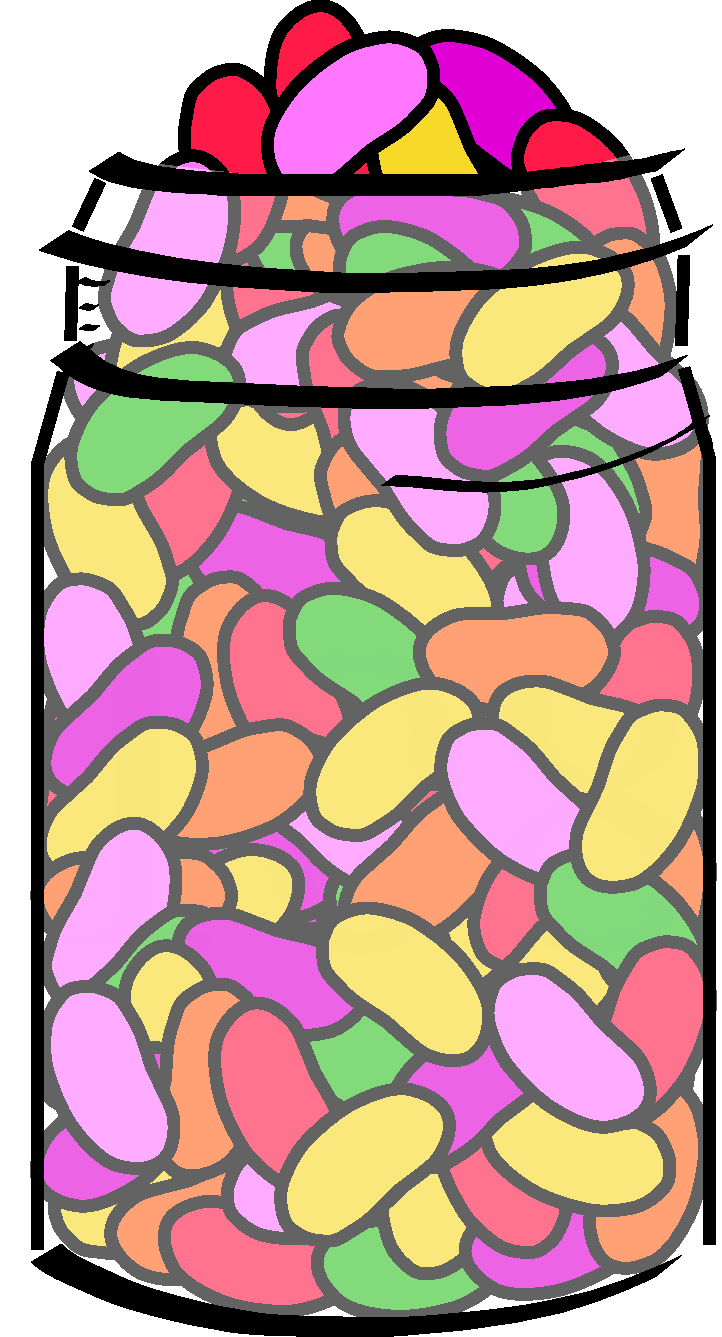
\includegraphics[width=0.25\textwidth]{figures/searches_beans.pdf}
\caption[
How many beans are in the jar?
]{%
How many beans are in the jar? This jar of jelly beans is a vehicle for our
discussion of inference and decision theory.
Please write your guess on this page.
The first correct answer wins a gold star.
}
\label{fig:searches_beans}
\end{figure}

\TODO{cut this}
Statistical data analysis suffers from dogma --- prescriptions and recipes that
students are taught to memorize and follow without knowing their reasons or
limitations.
From a standard undergraduate physics education, my experience has been
error propagation formulae,
least-squares fitting routines,
chi-squared per degree of freedom,
and myriad statistical tests and confidence intervals.
Many of these are effective approximations, but all also fail if misused
outside their domain.%
\footnote{%
Multiplicative error propagation is an example.
For $a = \mu_a \pm \sigma_a$ and $b = \mu_b \pm \sigma_b$,
the standard perturbative approximation for their product is
\(
\widetilde{\sigma}_{ab}
= \mu_a \mu_b \sqrt{\sigma_a^2/\mu_a^2 + \sigma_b^2/\mu_b^2}
% = \sigma_a^2 \mu_b^2 + \sigma_b^2 \mu_a^2
\),
but a calculation with their moments derives the exact result
\(
\sigma_{ab}
= \sqrt{(\mu_a^2 + \sigma_a^2)(\mu_b^2 + \sigma_b^2) - \mu_a^2\mu_b^2}
% = \sigma_a^2 \mu_b^2 + \sigma_b^2 \mu_a^2 + \sigma_a^2 \sigma_b^2
\)
if $a$ and $b$ are independent.
Since $\sigma_{ab}^2 = \widetilde{\sigma}_{ab}^2 + \sigma_a^2 \sigma_b^2$, the
propagation formula works only for small relative errors.
}
All effective methods of data analysis can be derived upwards from the roots of
probability and decision theory, and as elsewhere in physics, by knowing the
derivations we can also know when each approximation should work and when it
needs replacing.

We begin with what probability is: at its most abstract, a probability a
proportion of stuff within a larger whole.
Probabilities useful because proportions have applications, and because they
can be manipulated and interrelated with a linear and intuitive algebra.
Probabilistic data analysis follows the ordinary structure of science ---
write down models that make predictions, test those predictions against data,
then update your models to refine their predictions.
For this process, likelihoods are particularly important because they describe
our predictions. But not everything is a likelihood.
The remainder of this section uses a standard example from High Energy Physics
to introduce this probabilistic structure and other parts of its technical
language.

\subsection{Probability, abstract}
A probability $\prob{b}{a}$ is a number that quantifies the proportion
of $b$ within $a$, and can be expressed as a ratio~\cite{axioms1010038}
\begin{equation}
\label{eqn:searches_prob_ratio}
\prob{b}{a} = \frac{m(b, a)}{m(a)},
\end{equation}
in which $m(x)$ is a measure (a non-negative quantity assigned to its
argument, such as mass of tea in a cup), and the comma `,' means `and'
(logical and or set intersection or any other equivalent operation).
To continue that example, $\prob{b}{a}$ could be a proportion of tea within
a spoon within a cup, where $m(b, a)$ measures the volume of tea in a
teaspoon that is partially submerged in the cup.%
\footnote{%
All probabilities are conditional in this definition; $\probc{b}$ alone does
not exist unless some conditioning information is implicit from context.%
}

Logic is an important application of probability, for which $a$ and $b$ are
interpreted as logical propositions and
$\prob{b}{a}$ is the degree to which $a$ implies $b$, with the limiting cases
that $\prob{b}{a} = 1$ when $a$ implies $b$, and $\prob{b}{a} = 0$ when $a$
contradicts $b$.
Indeed, Cox's theorem derives the laws of probability by requiring compatibility
with Boolean logic~\cite{
cox1946probability,
cox1961algebra,
garrett1998nand,
jaynes2003probability,
keynes1920treatise
}.
Probability works for logic, and it works \emph{for tea, too}.

Probability \emph{distributions} $\prob{b}{a}$ spread unit probability mass
across states $b$, and need not be random distributions of fluctuating
$b$s~\cite{jaynes2003probability,frankfurt2005on}, although random processes
are useful applications.

Two algebraic rules derive from Equation~\ref{eqn:searches_prob_ratio}:
a \textbf{product rule}
\begin{align}
\prob{c, b}{a} &= \prob{c}{b, a}\times \prob{b}{a},
\label{eqn:searches_product_rule}
\intertext{%
that describes nested proportions
(perhaps a spoon within a teacup within a sink),
and a \textbf{sum rule}%
}
\prob{c\vee b}{a} &= \prob{c}{a} + \prob{b}{a} - \prob{c, b}{a},
\label{eqn:searches_sum_rule}
\end{align}
that describes combination in a union $\vee$ that coincides with logical `or'.
The subtraction avoids double-counting of any overlap, and is often avoided by
splitting any problem into orthogonal, or disjoint states.
For disjoint cases with labels $b_i$, normalization therefore requires that
\begin{equation}
\label{eqn:searches_normalization}
\sum_i \prob{b_i}{a} = 1.
\end{equation}
These rules are basic and well known, but we state them here to support the
following statements of how probabilities can be applied for practical
results.%
\footnote{%
The formulation with sums and products is not strictly unique, but all
alternatives are equivalent up to an invertible
transformation~\cite{axioms1010038}.
This choice is usually best because it uses ordinary addition and
multiplication.
In numerical analysis, however, it is often practical to use $\log$
probabilities to avoid overflows outside the range representable by floating
point numbers, thus changing multiplication to addition and addition to
the `$\log$-add-$\exp$' operation.
}

\subsection{Probability, applied}
\label{sec:searches_probability_applied}
\begin{figure}[tp]
\centering
\begin{subfigure}{\textwidth}
\centering
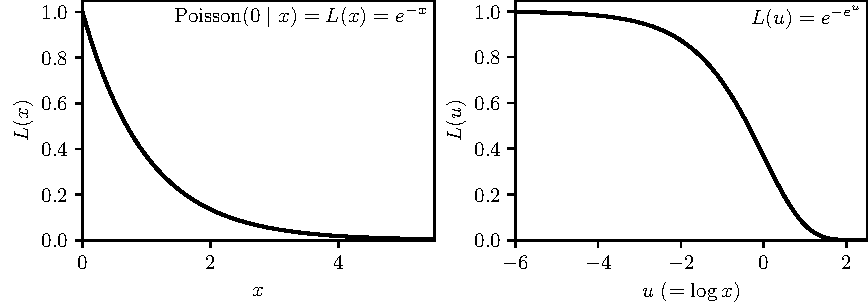
\includegraphics[width=\textwidth]{figures/searches_abacus_likelihood.pdf}
\caption{%
Likelihood: $\mathrm{Poisson}(0\mid x)$ in
(left) $x$ and
(right) $u = \log x$%
}
\end{subfigure}
\\[.5em]
\begin{subfigure}{\textwidth}
\centering
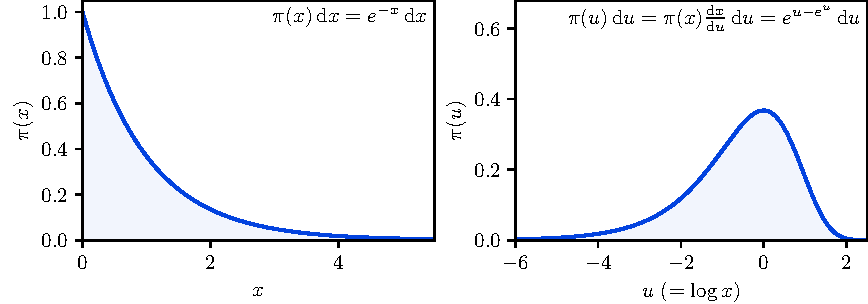
\includegraphics[width=\textwidth]{figures/searches_abacus_prior.pdf}
\caption{%
Prior: exponential density in
(left) $x$ and
(right) $u = \log x$%
}
\end{subfigure}
\caption[
Likelihoods and prior densities' transformations with coordinates.
]{%
Likelihoods and prior densities' transformations with coordinates.
The $\mathrm{Poisson}(0\mid x)$ likelihood and exponential $e^{-x}\mathrm{d}x$
prior have the same form (left), but the prior density changes to preserve its unit
area relative to $u = \log x$.
On changing to $\log$ coordinates (right), the likelihood slides horizontally,
but the prior density scales to preserve area.
Both maximum likelihood points are equal, but the maximum prior density moves.
\\[.5em]
Particle lifetimes follow exponential distributions and their maximum
densities are at zero time, but it is incorrect to describe their most probable
lifetimes as zero ---
the `most probable' $\log$ lifetime is not $\log 0$, but equals the mean
lifetime.
\\[.5em]
For zero Poisson data, the maximum likelihood rate is zero, but zero might not
be the most probable rate (if, for example, an experiment has known backgrounds).
}
\label{fig:searches_abacus}
\end{figure}
% science snake
Science involves making predictions, testing those predictions against data,
and reporting what is learned from the results.
Various probabilities are involved in this prediction and learning that have
conventional names to communicate what we intend to do with them.
Most important for prediction is a \textbf{likelihood}
\begin{align}
L(a) &= \prob{b}{a} \\
\label{eqn:searches_likelihood}
\intertext{%
that explores the probabilities assigned to a fixed result $b$ from different
contexts $a$, or how well different hypotheses predicted a result.
A likelihood is clearly a probability, but it is not a probability distribution
--- only the left hand argument $b$ forms a normalized distribution.
Alternatively, fixing the context gives a \textbf{prior}%
}
\pi(b) &= \prob{b}{a}
\label{eqn:searches_prior}
\end{align}
for fixed $a$, which is a normalized probability distribution over $b$.

Since prior probabilities are normalized distributions, it is usually
convenient to represent them as density functions.
Densities are stated relative to coordinates (or occasionally measures),
so changing coordinates changes their values as their unit probability mass
is sloshed around.
Likelihoods are not densities in the conditioning variable that they explore,
so changing coordinates slides them horizontally like beads on an abacus,
but does not change their values for equivalent states.
Figure~\ref{fig:searches_abacus} illustrates this difference.

Likelihood and prior are evidently related --- they explore two indices into
the same object, two sides of the same coin, and are assigned by the same
principles.
But they are profoundly different objects that work for different purposes,
and clarity in their distinction will help in our later understanding of
practical methods.
We use likelihoods to compare which hypotheses predicted observed data better
than others.
Prior to observing data we use priors to describe what might result from
different models; priors on data can be useful in designing our experiments,
and priors on other states describe other predictions.

To illustrate this, consider a histogram that bins event yields in
$\met$, with distributions from background and (supersymmetric) signal samples
overlaid.
Example such histograms are displayed in
Figure~\ref{fig:searches_sig_bkg_prior_likelihood}.
Since these histograms are normalized to unit area, they show prior
probability distributions along the bin axis; there is one prior
for events from each of the background and signal hypotheses.
Priors distribute unit probability explore along the bin axis.
In each bin, however, a likelihood function compares the assignments from
the two hypotheses: signal and background.
Likelihoods explore vertically down the sample axis.

\begin{figure}[tp]
\centering
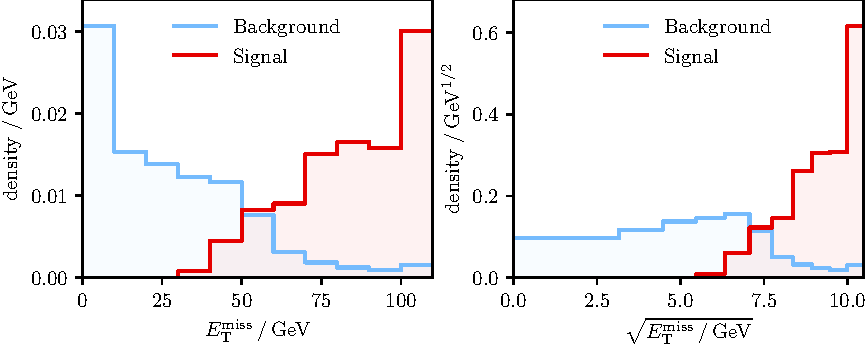
\includegraphics[width=\textwidth]{figures/searches_sig_bkg_prior_likelihood.pdf}
\caption[
Background and signal prior densities
]{%
Background and signal prior densities in $\eV[G]$ and $\eV[G]^{1/2}$ units.
When changing coordinates, probability mass moves as a fluid of constant total
volume, changing its shape in this density view to keep the area of the
rectangle in each bin constant.
A likelihood function indexes each bin in the background--signal labels,
and is independent of the coordinates units, since the area in each bin is
invariant.
}
\label{fig:searches_sig_bkg_prior_likelihood}
\end{figure}

Identical distributions are drawn in two different coordinates
on the left and right of Figure~\ref{fig:searches_sig_bkg_prior_likelihood};
they are identical in content, but differ in appearance because they use the
standard approach of representing each prior distribution as a density.%
\footnote{%
Density is a somewhat misleading term here.
Probability mass does not compress, it moves and redistributes --- it is more
like depth of tea than density of air.%
}
To preserve the area of each bin, which shows its probability mass,
bin heights therefore change to adapt to their widths that change due to the
differing values of $\met$ and $\sqrt{\met}$.
This coordinate-dependence of the prior density means that its maximum is
not always meaningful.
Since the probability mass in each bin is constant, the likelihood is
coordinate-independent.

One typically approximates such histograms by Monte Carlo simulation methods,
since simulations do not generate bin indices but event variables that derive
from the sampled events.
To connect these concept with probabilities, we begin with some notation;
we have hypotheses $h$ (signal or background),
a parameter $x$ that we histogram ($x = \met$),
and we observe a datum $d$ that datum indexes the histogram bins --- supposing
an event is observed in the overflow bin, it says
$d = `x > 100\,\eV[G]\textrm{'}$.
This observed bin has a likelihood function
\begin{equation}
L(x) = \prob{d}{x, h} = \prob{d}{x} =
\left\{
\begin{matrix}
1 & \textrm{if }~x > 100\,\eV[G], \\
0 & \textrm{otherwise} \\
\end{matrix}
\right.
\end{equation}
that corresponds to Equation~\ref{eqn:searches_likelihood} by
$b \leftarrow d$ and $a \leftarrow `x, h\textrm{'}$,
and simplifies $\prob{d}{x, h} = \prob{d}{x}$ since such binning is independent
of hypothesis.%
\footnote{%
Independence of the likelihood function from prior hypotheses is so common
that it should usually be assumed unless otherwise stated.
}
This example of a binary selection highlights how the likelihood acts as a
filter that rejects events that are contradicted by the data.
Other likelihoods that are not binary act similarly, but as inefficient filters
that reject events with some probability.

Simulating events from background and signal hypotheses samples from their
respective priors
\begin{equation}
\pi(x) = \prob{x}{h}
\end{equation}
that correspond to Equation~\ref{eqn:searches_prior} by
$b \leftarrow x$ and $a \leftarrow h$.
Although we previously used the same labels $a$ and $b$, those are only
labels --- the words `prior' and `likelihood' state our intent to index into
the left and right arguments, respectively.

When we fill a histogram by summing weights of simulated samples, we are
calculating another likelihood over hypotheses $h$ alone, not $`x, h\textrm{'}$
jointly.
To disambiguate the two, we call this abstracted, $x$-independent likelihood
the \textbf{evidence} $Z(h)$ for hypothesis $h$.
The evidence is calculable as
\begin{align}
Z
= \prob{d}{h} &= \sum_i L(x_i) \,\pi(x_i)
\label{eqn:searches_evidence_integral_sum}
\\
&= \int\! L(x) \,\mathrm{d}\pi(x),
\label{eqn:searches_evidence_integral_measure}
\end{align}
where Equation~\ref{eqn:searches_evidence_integral_measure} is notation for
integrating the likelihood function over the prior measure~\cite{
billingsley2008probability,
skilling2010foundations
}, and relates most closely to our practice of simulating from the model and
counting events that hit the non-zero likelihood in the bin.
We shall shortly derive this identity.
The name `evidence' relates to its application for model
comparison~\cite{mackay2003information}.
Supposing we have this one event with $\met > 100\,\eV[G]$, did it come from
the background or signal sample?%
\footnote{%
Questioning the origin of individual events is unusual in our context in
\atlas, but is done in other research into rare effects such as neutrino
interactions and black hole mergers~\cite{
opera2010event,
icecube2020event,
Abbott2021event
}.%
}
The answer depends on the signal and background cross-sections in our collider,
but larger evidence for signal does influence any conclusion to move in its
favour.

This expression as an integral --- an average over the prior, means that
the evidence $Z$ depends on what fraction of samples hits large values of
the likelihood function, and not only on how large that likelihood gets.
In contrast, one could consider a maximum likelihood approach that would
constrain a numerical optimization to regions of non-zero prior in each model.
Such optimizations can give useful upper bounds on the evidence, but this
example highlights a flaw when both models support the $\met > 100\,\eV[G]$
bin.
Then, both support the same maximum likelihood of
$L(\varepsilon + 100\,\eV[G]) = 1$, despite different evidence values.

% posterior
Perhaps we now want to see where in the overflow bin this event landed, and
compare the signal and background distributions there.
This is an inspection of the \textbf{posterior}
\begin{equation}
p(x) = \prob{x}{d, h} = \frac{L(x)\,\pi(x)}{Z},
\end{equation}
which is a prior probability distribution specialized by the data;
it simply uses the likelihood to filter simulated samples
(perhaps in `skimming an ntuple')
and re-normalizes them to a probability distribution within the constraint.

We finally have the four parts of `Bayesian' data analysis:
the two inputs \textbf{likelihood} and \textbf{prior},
and two outputs \textbf{posterior} and \textbf{evidence}.
These relate through Bayes' rule, which is a consequence of the
produce rule of Equation~\ref{eqn:searches_product_rule} and the
commutativity of `and' --- that `$a$ and $b$' is equivalent to
`$b$ and $a$';
the joint probability of data and parameters has two identical
forms, $\prob{d, x}{h}$ and $\prob{x, d}{h}$, that each factor into two
pieces:
\begin{align}
\prob{d}{x, h}\times \prob{x}{h} &= \prob{x}{d, h}\times \prob{d}{h},
\intertext{all of which we have named:}
\underbrace{L(x)}_\textbf{likelihood}
\times
~\,
\overbrace{\pi(x)}^\textbf{prior}
~\,
&=
\overbrace{p(x)}^\textbf{posterior}
\times
\underbrace{Z}_\textbf{evidence}
.
% \textbf{likelihood} \times \textbf{prior}
% &= \textbf{posterior} \times \textbf{evidence} .\nonumber
\end{align}
This is (the infamous) Bayes' rule, derived as a consequence of the
symmetry of logical `and' and the product rule of probability
algebra.

How Bayes' rule \emph{should} be used in scientific data analysis is to extract
useful information from the data.
If the likelihood function itself is interpretable, then it should be reported
directly.
When it is not, perhaps due to a complicated parametric modelling, then one
should abstract those parameters away to summarize the likelihood.
Properties such as local maxima or regions in which it exceeds meaningful
thresholds can be useful.
Evidence values for predictive models can also be useful if those models are
clearly stated and relevant to readers' interests.
Data act only through the likelihood function, and reporting a posterior
can act to obfuscate those data.

Posterior probabilities are, however, useful when digesting data to make
inferences about the world.
Reporting likelihood functions and evidence values allows readers to assign
priors as they wish.
For model comparison, for example between background $h_1=B$ and signal $h_2=S$
models, the analysis is conveniently linearized by expressing it in $\log$
ratio form:
\begin{equation}
\label{eqn:searches_log_odds}
\hphantom{\quad \quad \mid\mid \mathrm{context}}
\Delta(d) =
\log\frac{\prob{S}{d}}{\prob{B}{d}}
=
\log\frac{\prob{d}{S}}{\prob{d}{B}}
+
\log\frac{\probc{S}}{\probc{B}}
\quad \quad \mid\mid \mathrm{context}
,
\end{equation}
where we use the double bar, $\mid\mid$, to refer to any contextual information
a reader might wish to include.
When the evidence ratio is independent of that context, as it usually is,
it factors out from the prior (odds) ratio.
In this sense, likelihood (or evidence) ratios are scale factors that update
any odds prior ratio by the same multiplication, and that on this $\log$ scale
that means just adding a constant.

As data are reported more precisely, likelihoods will often tend towards zero
--- in the continuum limit, the probability of any data value vanishes.
Small likelihoods are themselves not significant unless other likelihoods
are larger --- unless other hypotheses predicted \emph{better}.
And these ($\log$) ratios can remain well-defined in continuum limits even as
both likelihoods tend towards zero~\cite{billingsley2008probability}.

From such $\log$ ratios, a little rearrangement recovers the individual
probabilities through the logistic function:
\begin{equation}
\label{eqn:searches_logistic}
\prob{S}{d} = \frac{1}{1 + e^{-\Delta(d)}}
.
\end{equation}
Physically, this is analogous to the Boltzmann distribution where the energy
of each model is its negative $\log$ probability, with unit inverse
temperature~\cite{
pmlr-v2-ranzato07a,
skilling2017david
}.
With multiple models in play, it is also called the `softmax'
function~\cite{MurphyKevinP.2012Mlap}.

The infamy of Bayes' rule stems from a fixation on the posterior distributions
from unjustified prior assignments.
Classical works by
Bayes~\cite{bayes1763lii} and
Laplace~\cite{laplace1774stigler} began this focus ---
both assume prior densities that are uniform in chosen coordinates, a practice
that can yield practical results in posterior inferences.
But to report scientific data, such practices are fairly criticized as
arbitrary when they influence the reported results.
Prior assignments are arbitrary.
You are welcome to propose any prediction in any circumstances, and the
scientific response is to test how well it predictts our observations of nature.
Our emphasis on the likelihood functions and evidence values that quantify
those predictions avoids the pitfall of seeking uninformative, neutral, or
unbiased priors by embracing priors as active and explicit predictions.
This is the modern, practical approach to Bayesian data analysis~\cite{
mackay2003information,
skilling2004nested,
skilling2006nested,
sivia2006data,
skilling2010foundations
}.

\begin{figure}[tp]
\centering

\includegraphics[width=0.65\textwidth]{figures/searches_baton_roue_bayes.jpg}
\caption[
Bayesian analysis produces two outputs: the evidence and posterior
]{%
Bayesian analysis produces two outputs: the
evidence $\prob{d}{h}$ and
posterior $\prob{x}{d,h}$ for hypothesis $h$, data $d$, and parameters $x$.
Posterior-only, semi-Bayesian methods are legitimately criticized because they
do not challenge the hypotheses that assign their priors $\prob{x}{h}$.
Since the evidence is a likelihood function over hypotheses, considering the
evidence can challenge those priors.
\\[0.5em]
Cartoon adapted from ``Baton roue'' by
Corentin~Penloup~\cite{penloup2011baton}.
}
\label{fig:searches_baton_roue_bayes}
\end{figure}

Some sources continue to define Bayesian analysis as the computation of
posterior probabilities given data, often without naming the evidence, and
expressing it only as the sum from
Equation~\ref{eqn:searches_evidence_integral_sum}
--- as just a normalizing constant~\cite{
Neyman1937Outline,
gelman1995bayesian,
gelman2008objections,
DAgostini:1994fjx,
DAgostini:2010hil,
cowan1998statistical,
pdg2022ynf
}.
Bayes' rule has two outputs, and both outputs have uses.
Cutting out the evidence hamstrings Bayesian analysis, leaving only the
semi-Bayesian posterior-only approach and its clear flaws.
A bicycle is stable with two wheels and falls over if one either
is removed;
Figure~\ref{fig:searches_baton_roue_bayes} illustrates this analogy.
Although it is possible to ride a unicycle, it is a circus trick and not often
a practical tool.

Phrased succinctly by Skilling~\cite{skilling2008rant},
``we SHOULD use Bayes by assigning subjective priors and inspecting evidence
values.''
This framing of probabilistic data analysis agrees exactly with our standard
practice of histogramming simulations,
as illustrated in Figure~\ref{fig:searches_sig_bkg_prior_likelihood}:
signal and background models define priors, and their (normalized) bin yields
are the evidence values that we use to compare the models.
Finally, their corresponding posteriors are the normalized shapes those samples
take within the observed histogram bin, with which we do not compare the
models, but which could in principle be used for secondary interpretations.

\subsection{Probability assignments}
Probability algebra manipulates probabilities, but does not state how they
should be initially assigned.
In general, such probability assignments are free and unconstrained, and might
be informed by calibration data or loosely motivated opinions.
But there are examples of unambiguously derived that are commonly used in
High-Energy Physics, notably the Poisson and Gaussian distributions.
To avoid turning this thesis into a textbook, we only sketch the derivations
of these, and refer to real textbooks for their detailed
derivations~\cite{jaynes2003probability}, both of which use the exponential
identity that
\begin{equation}
\label{eqn:searches_exponential}
\exp(x) = \displaystyle \lim_{N \to \infty}
\left(1 - \frac{x}{N}\right)^N
.
\end{equation}

The Large Hadron Collider collides $40$~million proton bunches per second,
but \atlas' trigger system accepts only around $1000$ of
those per second~\cite{atlas2020trigger}.
This means that we have a scenario with a large fixed number $N$ of trials
(bunch collisions)
and a small probability of binary acceptance (triggering),
due to a notable collision event.
The summed total number $n$ of accepted events is therefore described by the
binomial distribution for $n$;
\begin{equation}
\label{eqn:searches_binomial}
\mathrm{binomial}(n\mid N, p) = p^n (1 - p)^{N - n} \times \binom{N}{n}
,
\end{equation}
which is a product of the probabilities (produce rule) in the sequence of $N$
accept/reject decisions, summed (sum rule) over all permutations of that sequence
that could have led to the total $n$.
With our tiny trigger rate, we are interested in the limit of small
$p$ and large $N$, which result in a mean acceptance number of $\lambda = Np$.
Using the exponential identity of Equation~\ref{eqn:searches_exponential}, one
can show that this limit tends towards the Poisson
distribution~\cite{jaynes2003probability};
\begin{equation}
\label{eqn:searches_poisson}
\mathrm{Poisson}(n\mid \lambda) = \frac{\lambda^n}{n!}\exp(-\lambda)
,
\end{equation}
which is used ubiquitously in the analysis of our histograms.

The Gaussian distribution has many justifications:
as the unique distribution that is spherically symmetric and factors linearly
into independent dimensions~\cite{
jaynes2003probability,
herschel1850normal,
maxwell1860normal,
muller1959note,
marsaglia1972normal
},
as a practical approximation that permits analysis in linear algebra,
and as the maximum entropy~\cite{PhysRev.106.620} distribution for a
known mean and variance.
This maximum entropy statement means that for a distribution with known mean
and variance in given coordinates, its best Gaussian approximation matches
those moments.\footnote{%
By `best', this statement means a minimal Kullback-Leibler divergence
\(
H(p\leftarrow q) = \sum_i p_i \log(p_i/q_i)
\)
from the Gaussian approximation $q$ to the target $p$ with known moments.
Such an approximation may not be \emph{good}, but it is best in class.%
}
As a limiting approximation, the Gaussian form arises from products of many
functions, such as combinations of many independent measurements that multiply
their likelihood functions.
At a maximum $\check{x}$, the first derivative of a function vanishes and the
second derivative is negative.
Taylor expanding about this maximum to the leading order, the product looks like
\begin{equation}
f(x)^N = \displaystyle \lim_{N \to \infty}
\left(
1 - \kappa (x - \check{x})^2
\right)^N,
\end{equation}
which, again by Equation~\ref{eqn:searches_exponential}, goes into the Gaussian
form
\begin{equation}
\label{eqn:searches_gaussian}
\mathrm{Gaussian}(x\mid \mu, \sigma)
\,\mathrm{d}x =
\frac{1}{\sqrt{2\pi \sigma^2}}
\exp\!\left(-\frac{1}{2}\frac{(x - \mu)^2}{\sigma^2}\right)
\mathrm{d}x
\end{equation}
where the prefactor is for normalization to a probability distribution over
$x$, and we include the $\mathrm{d}x$ terms as reminders that it is a density
function in $x$, not a probability exactly.
On a $\log$ scale, the Gaussian form is simply quadratic in $\mu$ (or $x$);
that quadratic form continues in its multivariate generalization, and
justifies least-squares methods.

Here, $\kappa$ and $\sigma$ both relate to the second derivative of the target
function; this relationship extends to multiple dimensions in the Hessian
matrix and its inverse, and allows one to estimate error bars from second
derivatives --- a practical tool that the methods discussed in this thesis
employ.

This is not the famous Central Limit Theorem, which is related to the
distribution of sums.
But can be used to derive it: the distribution of a sum is a convolution, which
becomes a product in Fourier-transformed space, and that product can converge
to a Gaussian function by this same derivation if the mean and variance exist.
A beautiful alternative proof of the Central Limit Theorem is given by
Jaynes~\cite{jaynes2003probability}
(Section ``7.16 The central limit theorem''), but would be spoiled by a
reproduction here.

\TODO{reduce this}
In the current year, it would be remiss to not mention machine learning
algorithms.
Among various other applications, learning algorithms demonstrate practical
successes in probability assignments, such as assigning
probabilities to labels for classification,
or to assign probabilities to words for text
generation, or any of myriad other
predictions~\cite{MurphyKevinP.2012Mlap, radford2019language}.
Machine learning tunes flexible functions by consuming data and testing their
predictions in the manner we have described; their training and testing works
roughly as follows:
\begin{enumerate}
\item Predict new data with $\prob{d_i}{f(d_{i-1}, \ldots), h}$.
Keep this evidence as a testing score for comparison against other models.
(Practically, keep its equivalent $\log$ mean over independent samples.)
These $d_i$ may be only reductions of the data, such as class labels
or index permutations~\cite{Noroozi2016jigsaw, multitaskself2017}.
Other inputs that are not predicted, such as associated images that the machine
uses to predict the labels, are included in the context $h$.
\item Use those data to update your state
$f(d_{i-1}, \ldots) \to f(d_i, d_{i-1}, \ldots)$.
Unlike ideal posterior updating, this encodes only a function of the data, not
its whole --- one usually cannot afford to consume all aspects of data, so
although theoretically suboptimal this approximation is vastly superior in
practice.
Learning only part of the data is not wrong, it is just less precise than a
divinely perfect learning algorithm, which we do not currently possess.
\item Go to 1.
\end{enumerate}
These sequential data $d_i$ might be labelled the `training', `validation',
and `testing' sets, but other splittings are possible.
This perspective highlights the importance of independent training and testing
sets --- since $\prob{d}{d, \ldots} = 1$, if any memory of $d_i$ is kept in
the $f(\ldots, d_i, \ldots)$ state, then it is a memory and not a prediction.
Independent testing data permit the evidence interpretation of predictive
probabilities.


\subsection{Decision theory}
Now that we have thoroughly covered probability theory, we are ready to return
to the jelly bean game that is illustrated in Figure~\ref{fig:searches_beans}
and asks you to guess how many beans are in the jar.
Given all you know about illustrations of jars and beans, you could make a
vague guess without looking.
That guess should only be refined after inspecting the image and updating your
model to account for it.
Although I do not propose that human brains \emph{do} use probability
algebra~\cite{jaynes1988brain}, this inference process could, in principle,
be modelled numerically by distributing probability over the positive integers
and updating those probabilities in light of a likelihood function for the
image data.
Any guess, however, does not depend only on that probability distribution,
but on the risks and rewards associated with guessing.

As written in the caption to Figure~\ref{fig:searches_beans}, there is a
notional reward to the first exactly answer.
You are therefore incentivized to answer a) quickly, before other good guesses,
and b) exactly, with no reward for being close to the true answer.
If you are the first to answer, then it makes sense to write what you think
is the most probable number.
But others following you, seeing your answer, should prefer to guess
differently if they want to win (and they think any other guess is plausibly
correct).

To try hard, you could even dissect the vector graphics of the figure and count
its bean objects, but that may not be optimal use of your resources --- the
dubious promise of a gold star may be worth little to you.

When considering what decision to make, it feels natural to consider what
might result from each possible action and to judge that action on how good or
bad its results would be.
Mathematical decision theory agrees with this intuition---
a famous theorem by Wald~\cite{
wald1947bayes,
wald1950bayes,
jaynes2003probability
}
shows that the optimal solution to any decision problem can be always be
formulated as the minimization of an expected cost function, or risk:
\begin{equation}
\label{eqn:searches_bayes_decision_rule}
R(t) = \int\! c(t, x) \,\mathrm{d}p(x)
,
\end{equation}
where we mean `expected' in the mathematical mean sense of the `mean' average.
This cost function $c(t, x)$ evaluates the badness of outcomes for a given
decision $t$ and states of the world $x$ to which context must assign prior
probabilities $p(x)$.
For a given cost function and prior, one should choose the decision $t$ that
minimizes $R(t)$.

Although alternative ideas (such as minimax, minimizing a maximum
loss~\cite{savage1951review}) can work well in certain contexts, this theorem
states that restricting oneself to minimizing an expected cost function cannot
deny one access to optimal decisions.
Alternative formulations can at best be equivalent.

This theory does not, however, define how to construct that cost function.
Like the prior, it must come from context, and indeed the two are intertwined
in the risk;
decision-making machines and organisms are capable of learning to make good
decisions without constructing either cost or prior explicitly.
Towards our goal of usefully reporting data, such decision theory has been
applied to argue for ways to quote properties of posterior distributions.
As examples, minimizing the expected absolute error $|x - \check{x}|$ leads
to reporting the median, and minimizing the expected square error
$(x - \check{x})^2$ leads to reporting the mean.
Had the rules of our bean counting game rewarded you based on such distances,
these results could have been good guesses. But those weren't the rules.

When arguing that we should report likelihoods and evidence values for our
data, we have not explicitly constructed cost functions, nor have we made
quantitative predictions of future events.
But we can qualitatively consider them in this decision theory framework ---
we imagine that future scientists will want to reuse our data, and would be
pleased (attain a small cost) if they were able to reinterpret the results for
their own models.
We can therefore reason that likelihoods would usually have more utility than
alternatives such as point posterior averages.

% connection to frequentist section
An amusing feature of Wald's theory is that it was formulated from a
perspective on probability in which,
``In most applications, however, not even the existence of an a priori
distribution can be postulated''~\cite{wald1950bayes}.
That might seem problematic, since the risk is the expectation value of a cost
function over a prior (or \emph{a priori}) distribution.
Wald was nonetheless interested in these decision rules for their
``completeness'' that he had proven, and named them ``Bayes'' decision rules
despite approaching the theory from a stalwart non-Bayesian perspective.

Although Bayes' rule is not seriously disputed, the system in which Wald was
working defined probability as a frequency in random sampling, which cannot
reasonably apply to subjective, non-random distributions of probability mass
that many prior distributions are.
This frequency-restricted, `frequentist', philosophy dominated 20th century
statistical research, and influences practices that \atlas\ continues to
employ.
We therefore review some features of frequentist statistics in the following
section.

\begin{singlespacing}
\section{Frequentist theory}
\label{sec:searches_frequentist}
\begin{epigraphs}
\qitem{%
Within this theory, statistical methods of great practical usefulness have been
developed, and its statements can and frequently do contribute in a vague way
to the interpretation of data. \ldots%
}%
{John~W.~Pratt,
\textit{Review: Testing Statistical Hypotheses},
1961~\cite{pratt1961testing}}
\end{epigraphs}
\end{singlespacing}

Probability as defined in Equation~\ref{eqn:searches_prob_ratio} is a
proportion of stuff within a larger whole, which when formalized as a ratio
of measures and has broad applications.
Frequentist theory confines itself to the special case where those measures
are numbers of randomly occurring events, such that a frequentist
probability is a ratio of frequencies:
\begin{equation}
\label{eqn:searches_prob_frequency_ratio}
\freq{b}{a} = \lim_{N \to \infty}\frac{n}{N},
\end{equation}
where $n$ is the number observed to satisfy conditions $a$ and $b$ when
$N$ have satisfied $b$.
Interpreted with the Binomial model of
Equation~\ref{eqn:searches_binomial}, this definition converges to our more
general probability whenever it applies.

We do think of many processes as random when considering scientific data, so
this definition works widely for likelihood functions.
Non-data hypotheses, however, are rarely considered as actually random events,
so the frequency definition cannot not apply.
Prior predictions often apply probabilities to express subjective uncertainties
that are manifestly non-random.
Under this frequency definition, those predictive probabilities are nonsense
and must be rejected.
The frequency definition does not change probability algebra, it only restricts
it to a permitted scope.

Coin tosses, for example, can be imagined as random.
Earth's human population could toss a few billion coins to precisely
establish a probability of landing heads from the ratio of
$n$ (number of heads) to $N$ (number of tosses).
Now suppose you are given a red envelope containing a coin;
which way up is the coin in the envelope?
You could guess or bet on the answer, and that decision might involve a tacitly
assumed probability.
A frequency, however, would only be permitted if the envelope had been packaged
at `random'.
Was the coin first tossed to randomize its face, or placed deliberately?
You do not know.
In Neyman's words,
``I have put the word ``~random~'' in inverted commas because it is very
difficult to define what is meant by it in practice''~\cite{
Neyman1937Outline
}.

Tom~Stoppard's play `Rosencrantz and Guildenstern Are Dead'~\cite{
stoppard1967rosencrantz
}
opens with a clearer example ---
the titular characters toss a coin ninety-two times, all landing heads.
They then play a game with a third player, landing eight more heads.
Will the next toss be heads or tails?
The answer is not random --- it is burned onto paper in print, so no frequency
can be assigned.
Were subjective probabilities permitted, you could predict the result, and that
prediction would be subjectively informed by it being the one-hundred-and-first
toss, our cultural entanglement with round numbers in base-10, and your reading
of these words.
Frequentist theory, however, forbids such subjective probabilities of
non-random unknowns, so is left to search for alternative modes of inference.

As established in Section~\ref{sec:searches_data_analysis}, the original
probability theory of Laplace and Bayes did not require frequency
interpretations; these were developed later in the 19th century by
mathematicians including Venn~\cite{venn1866logic} and
Boole~\cite{boole1854investigation}, in reactions that may well have been
propelled by reactions to flawed posterior-only methods.
Modern frequentist theory has a rigorous set-theoretic formulation in the
Kolmogorov axioms~\cite{
kolomogoroff1933de,
kolomogoroff1950translated,
Neyman1937Outline,
axioms1010038
}, but \emph{applied} frequentist methods are constrained with considerably less
precision --- the denial of certain (non-frequency) probabilities does not
construct their replacements, and various surrogates have evolved.

Modern frequentist methods are largely attributable to work by
Ronald~Fisher (for likelihood, $p$-values, and estimation criteria~\cite{
fisher1912fitting,
fisher1915frequency,
fisher1921probable,
fisher1922estimators,
fisher1925smrw,
fisher1956statistical
}),
and Jerzy~Neyman and Egon~Pearson
(for statistical hypothesis testing and confidence intervals~\cite{
neymanpearson1933lemma,
neymanpearson1928max
})
in the 1920s and '30s.
These Fisher and Neyman-Pearson schools do not form a unified framework, but
do comprise a collection of ideas and practices that survive in modern science,
and which explain some methods, to be introduced in
Section~\ref{sec:searches_practice}, that we apply to modern LHC data.

Some literature names this Fisher/Neyman-Pearson assemblage
``classical'' statistics~\cite{
Neyman1937Outline,
lehmann2011fisher,
Feldman:1997qc
}, but that is simply inaccurate for 20th century creations that innovated on
18th century ideas~\cite{bayes1763lii, laplace1774stigler}.
Jaynes instead names them ``orthodox''~\cite{
Jaynes1976intervals,
jaynes2003probability
},
which may have been accurate in his environment, but different
(heretical?) ideas have taken hold in research at the LHC ---
the orthodoxy has moved on.
We therefore stick with `frequentist'.

\begin{figure}[tp]
\centering
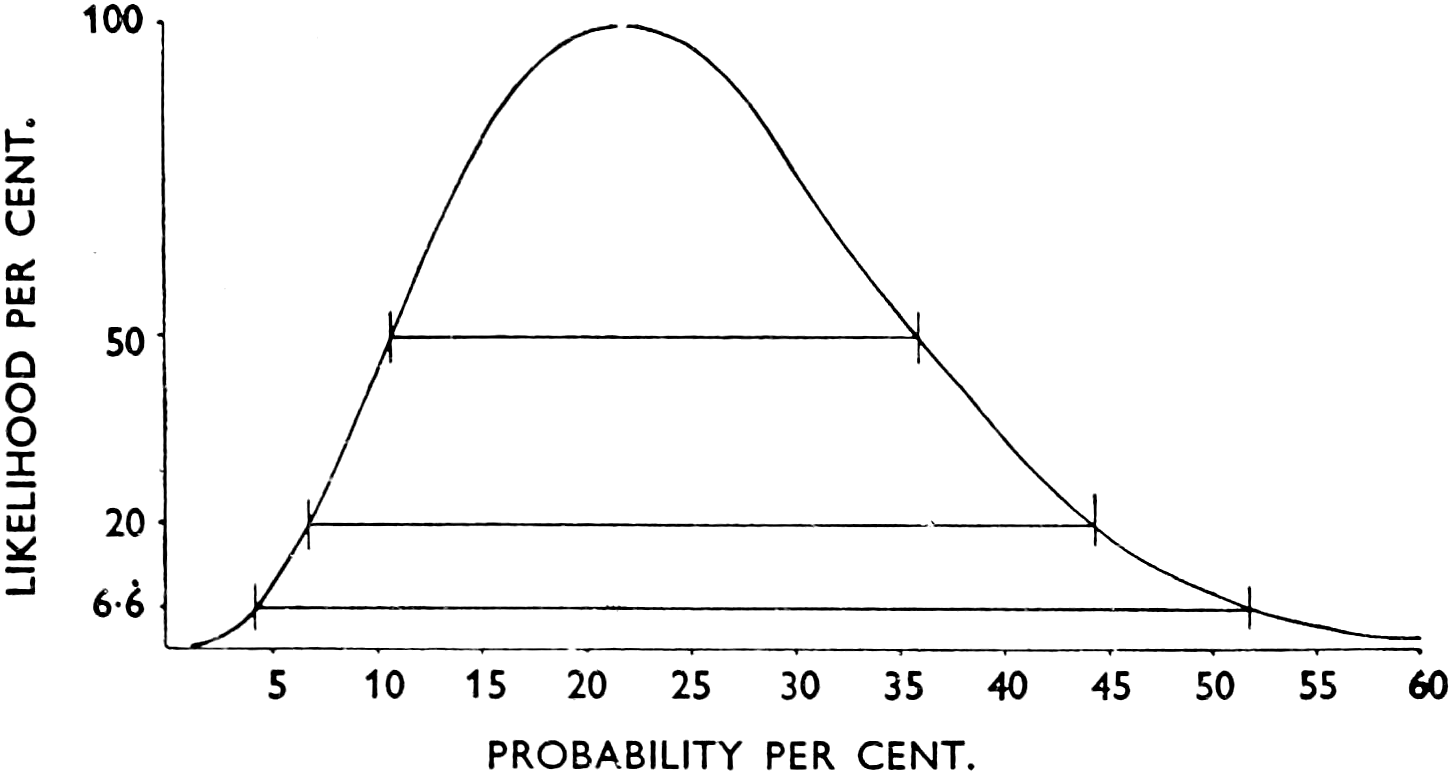
\includegraphics[width=0.95\textwidth]{figures/searches_fisher_likelihood_binomial.png}
\caption[
Intervals exceeding ratios from the maximum of a Binomial likelihood function,
reproduced from Fisher
]{%
Intervals exceeding ratios from the maximum of a Binomial likelihood function,
reproduced from Fisher~\cite{fisher1956statistical}.
Horizontal lines mark regions where the likelihood function exceeds
$1/2$, $1/5$, and $1/15$ of its maximum, respectively.
The extents of these lines could be tabulated to usefully communicate aspects
of its profile.
}
\label{fig:searches_fisher_likelihood}
\end{figure}

\subsection{Fisher}
\label{sec:searches_fisher}
% likelihood
Fisher coined the term `likelihood'~\cite{
fisher1912fitting,
fisher1915frequency,
fisher1921probable,
fisher1922estimators
} in the usage that
we employ for the probability of observed data given varied
contexts%
\footnote{%
Fisher used the term `likelihood' for the function exploring
contexts and `probability' for the distribution over
outcomes~\cite{fisher1925smrw}.
We choose the alternative word `prior' for his `probability' since the
likelihood is also a probability, just not a probability \emph{distribution}.
},
and deserves credit for popularizing its use in interpreting and communicating
data without the confounding influence of prior probabilities.
In his own words,%
\begin{displayquote}
\small
``%
We can know nothing of the probability of hypotheses or hypothetical
quantities.
On the other hand we may ascertain the likelihood of hypotheses
and hypothetical quantities by calculation from observations%
''~\cite{fisher1921probable},
\end{displayquote}
and furthermore we agree that in comparison to other prescriptions
(specifically confidence intervals, to be introduced in
Section~\ref{sec:searches_np}),
\begin{displayquote}
\small
``%
For all purposes, and more particularly for the \textit{communication} of the
relevant evidence supplied by a body of data, the values of the Mathematical
Likelihood are better fitted to analyse, summarize, and communicate
statistical evidence of types too weak to supply true probability statements%
''~\cite{fisher1956statistical}.
\end{displayquote}
For example, Figure~\ref{fig:searches_fisher_likelihood} displays a figure by
Fisher~\cite{fisher1956statistical} that illustrates how data can be usefully
reported by the likelihood's maximum and the regions in which it exceeds
certain ratios relative to that maximum.%
\footnote{%
We use such $L(\check{x})\pm\mathrm{ratio}$ visualizations for
$\pm1\sigma$ and $\pm2\sigma$ error bars on Poisson data in
Figure~7 of~\cite{lester2022hunting}.
When recommending error bar recipes, \atlas' statistics committee appears
to have not considered this option~\cite{cowan2011errorbars}, although
our statistics experts are surely familiar with Fisher's work.
}
That the likelihood contains all relevant information in the data is true by
definition in our formulation of Equation~\ref{eqn:searches_log_odds},
but non-Bayesian arguments find the same conclusion~\cite{
birnbaum1962foundations,
savage1962foundations
}.

Maximum likelihoods are often useful for interpreting and communicating data.
The location of a maximum likelihood can be a useful estimate for the
parameters being considered, and Fisher showed that maximum likelihood
estimates satisfy some desirable criteria~\cite{fisher1922estimators}.
These criteria do not include \emph{unbiasedness}, which states that the mean
value of an estimate --- over the distribution for alternative data --- should
equal its known true value~\cite{
sheynin1989aa,
Neyman1937Outline,
pdg2022ynf
}.
Defining bias as a difference from a mean fails to be coordinate-invariant,
so an unbiased estimate of the variance $\bar{\sigma}^2$ is a biased
estimate of the standard deviation $\bar{\sigma}$ --- the square of the mean
is not the mean of the squares~\cite{barlow2019svl}.
Fisher rejected the bias criterion for this
reason~\cite{jaynes2003probability}, and other definitions absorb its
arbitrariness into an explicit loss function~\cite{lehmann2005testing}.
Requiring unbiasedness can actively harm our results by preventing the use of
useful estimates,%
\footnote{%
Problem~1.14 of~\cite{lehmann2005testing} has a delightful example of
estimating an exponentiated a Poisson mean $e^\mu$ from $n$ data
where the unique unbiased estimate is $(-1)^{n + 1}$.
Section~17.3 of~\cite{jaynes2003probability} finds similar nonsense for
unbiased estimates of $\mu^2$ and $\exp(-\mu)$.%
}
or by obfuscating those estimates with bias corrections.
Remaining uses of unbiasedness in High Energy Physics~\cite{
pdg2022ynf,
Tullythesis,
lhcb2018563,
LHCb:2021trn,
LHCb:2015yax
}
are largely explained by the linguistic trickery of its name --- our
results should not be biased by forces outside the data and relevant theory,
and we like to report that to be true.
But we should proudly proclaim that our results are `biased' under this flawed
statistical definition if that makes them better by any reasonable measure.

% likelihood quotes
In avoiding the pitfalls of reported posteriors, Fisher's use of likelihoods
remains innovative and practical.
However, the hard rejection of priors on hypotheses also prevents evidence
calculations, without which likelihoods alone become confounded in many
parameters, perhaps making them nuisances.
To circumvent this, frequentist methods employ two key concepts:
test statistics, which can reduce the data to remove unwanted parameters,
and $p$-values, which divert the discourse
from what the alternative hypotheses \emph{are}
to what alternative data \emph{might have been}.

% test statistics
A statistic is a function of data, and a test statistic is just a statistic
that is used in statistical tests.
For \atlas\ collision data, event variables are statistics; when working with
data, one always uses statistics and is free to design them for their benefits
in context.
Just as we define event variables (like $\pt$) to remove nuisance
dependencies (on $\phi$ rotations or longitudinal boosts),
useful test statistics can also eliminate unwanted parameters.
The quintessential example is the $t$-statistic,
\begin{equation}
\label{eqn:searches_t_statistic}
t(d) = \frac{\bar{\mu}(d) - \mu}{\bar{\sigma}(d)}\sqrt{n}
,
\end{equation}
which shifts the sample mean $\bar{\mu}(d)$ by a known true mean $\mu$, and
scales that difference down by the same standard deviation
$\bar{\sigma}(d)$~\cite{student1908, fisher1925t}.
By dividing out a (scale-equivariant) estimate of the standard deviation, $t$
is independent of common scale factors on the data, and that scale invariance
has helped to drive the study and common use of this
$t$-statistic~\cite{lehmann2011fisher}.

One can usefully reduce observed data to just the test statistic
$\tilde{t} = t(d)$, and compare likelihoods on that observed $\tilde{t}$
to compare how well different hypotheses predict it.
For unclear reasons, Fisher advocates a different use ---
rather than considering likelihoods and likelihood ratios, he recommends
that researchers consider the ``probable error''~\cite{fisher1921probable},
which is a cumulative distribution function in the negated test statistic.
In modern jargon, a `probable error' at the observed test statistic
$\tilde{t}$ and an hypothesis $h$ is a \textbf{\pvalue}
\begin{align}
P(h)
&= \prob{t \geq \tilde{t}}{h}
\label{eqn:searches_pvalue}
\\
&= L(h) + \prob{t > \tilde{t}}{h}
\label{eqn:searches_pvalue_likelihood}
;
\end{align}
the \pvalue\ $P(h)$ is the prior probability of data
\emph{greater or equal to} the observed data when ordered by the value of the
test statistic.
Equation~\ref{eqn:searches_pvalue_likelihood} points out that the \pvalue\ is
just is the likelihood plus some fluff from a tail of larger test statistics.

Fisher illustrates the use of \pvalues\ in the second example
of~\cite{fisher1921probable}, which models some data with a parameter $r$ and
compares two hypotheses
$r=0.3$ and
$r=0.95$, finding $p$-values
$P(r=0.3)=0.142$ and
$P(r=0.95)=0.00014$.
``Thus'', Fisher concludes, ``the value $0.95$\ldots\ is roughly $1000$ times
less likely than $0.30$''
(``when measured on the $r$ scale'').
By writing `likely', Fisher is carefully not referencing the probability
of parameters, but their likelihoods in our definition.
But this factor of $1000$ is a \pvalue\ ratio, not a likelihood ratio,
so how can this make sense?
Plausibly, it results from a tacit data reduction; comparing
Equations~\ref{eqn:searches_pvalue} and~\ref{eqn:searches_likelihood}
shows that the \pvalue\ is a likelihood only if the result is reduced from
$A: t =    \tilde{t}$ to
$B: t \geq \tilde{t}$.
And since this reduction is technically true --- $A$ implies $B$ --- the
likelihood ratio on $B$ is logically valid and not \emph{necessarily}
misleading if accurately reported.

However, $B: t \geq \tilde{t}$ is a logical statement (true for all test
statistics greater than or equal to the observed value) and not a randomly
occurring event; it therefore does not have a frequentist probability and so
is probably not what Fisher intended.
Much more importantly, the reduction to a one-sided inequality has no tangible
benefit --- it reduces the information content of the reported data without
reducing the associated costs of reporting or interpreting those data.
Both $A$ and $B$ are printed in the same number of characters, and $p$-values
can be painfully expensive to evaluate.
And it actively harms any result with small a test statistic by
diluting the likelihood ratio, since if
\begin{equation}
\log \frac{L(h_1)}{L(h_2)}
\to
\log \frac{
L(h_1) + \prob{t > \tilde{t}}{h_1}
}
{
L(h_2) + \prob{t > \tilde{t}}{h_2}
}
\end{equation}
then large tail probabilities squash the $\log$ likelihood ratio toward zero.

Fisher's \pvalue\ ratio of $1000$ is, therefore, a $\log$ likelihood
ratio of $+6.9$ in favour of $r=0.3$ over $r=0.95$, which is a moderately
strong  indication of roughly $3.7\sigma$.
But a likelihood ratio on the test statistic itself, and not the inclusive
tail statement, would encode strictly more information and could provide a
more precise answer.

\begin{figure}[tp]
\centering
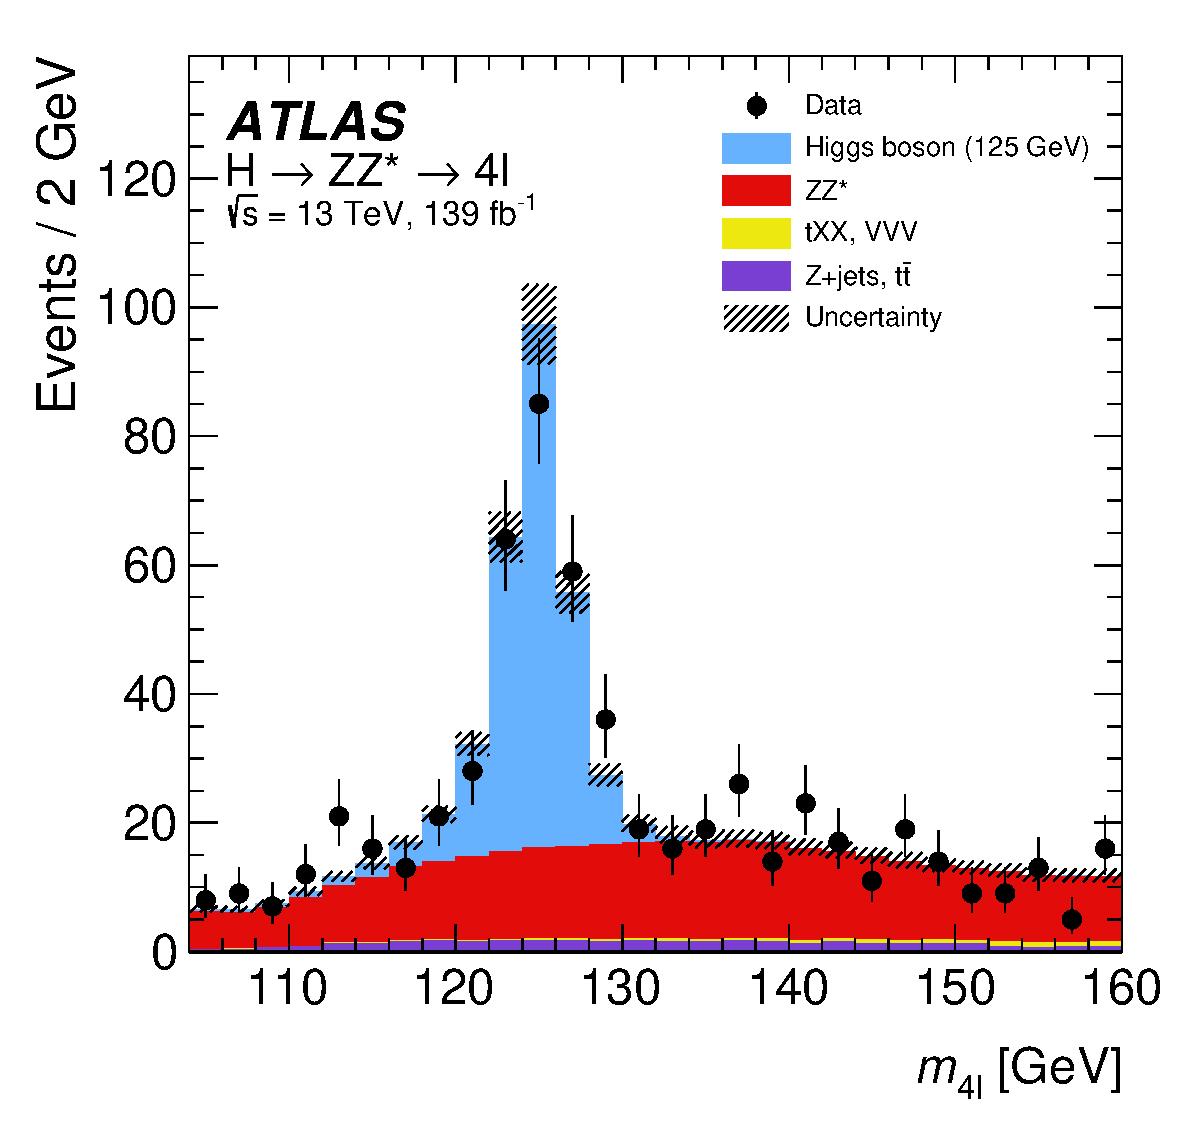
\includegraphics[width=0.6\textwidth]{figures/searches_atlas_higgs_4l_2207_00320.pdf}
\caption[
Signal and background distributions reproduced from the recent \atlas\
measurement of Higgs boson decays to $4\ell$
]{%
Signal and background distributions reproduced from the recent \atlas\
measurement of Higgs boson decays to $4\ell$~\cite{ATLAS:2022net}, with
observed data.
This example illustrates \pvalues\ pathological dependency on tail selections,
and the benefits of likelihood ratios.
}
\label{fig:searches_atlas_higgs_4l}
\end{figure}

Fisher claims that the \pvalue\ indicates the ``significance'' of an
observation~\cite{fisher1925smrw}, with small or large values being
suspiciously significant, and that
``If $P$ is between $.1$ and $.9$ there is certainly no reason to suspect the
hypothesis tested.''~\cite{fisher1925smrw}
This may have been true for his intended applications, but it is not general;
as for other likelihoods, small values are only meaningful in comparison
against larger values from alternative hypotheses on the same data.

Consider for example the distributions of signal (Higgs boson) and background
(mostly $ZZ^*$) samples in Figure~\ref{fig:searches_atlas_higgs_4l}.
If an event is observed at $m_{4\ell} = 125\,\eV[G]$, is it signal or
background?
It is obviously a Higgs boson candidate, but $m_{4\ell}$ is around the middle
of both signal and background distributions, so with an $m_{4\ell}$ test
statistic $P(\textrm{Higgs boson}) \approx P(ZZ^*) \approx 0.5$, so neither
is ``suspect''.
Local ratios between the two distributions clearly favour signal for this
event, however; the $p$-values' failure is in their dependence on irrelevant
tail areas, which are a feature of the histogram and not the data.
This $ZZ^*$ density peaks for $ZZ$ above a
$2 m(Z) \approx 180\,\eV[G]$ kinematic edge,
and $Z \to 4\ell$ around $m_{4\ell} \approx m(Z)$;
expanding the histogram to show either of these tails would change nothing
local to our $m_{4\ell} = 125\,\eV[G]$ event, but would change our $p$-values.

Better test statistics can soften this problem, and a key observation by
Neyman and Pearson is an optimality of likelihood ratio test statistics.


\subsection{Neyman-Pearson}
\label{sec:searches_np}
Suspecting an hypothesis when its \pvalue\ lands below (or above) a threshold
means that there is a prior probability $\alpha$ that any hypothesis will be
suspect after an experiment.
For example, in Fisher's suggestion of $P(h) \in 0.1--0.9$ being not suspect,
then $\alpha = 0.2$.%
\footnote{%
Matching $\alpha$ can be impossible in discrete distributions if
the tail probability masses do not add exactly to $\alpha$.
Neyman accommodates this by allowing inequalities with $\alpha$~\cite{
neyman1935Intervals
}.
Other approaches introduce ``extraneous randomization'' to
break up discrete distributions~\cite{tocher1950discontinuous}.
This problem of inexact `coverage' continues to cause controversy~\cite{
Read2002cls,
Feldman:1997qc,
cousins2008evaluation,
Cranmer2006Statistical
}.%
}
otherwise meets the edges at $0.1$ and $0.9$ in its cumulative distribution).
And that chance is independent of the hypothesis, its alternatives, and even
the nature of the experiment.

Obediently followed, these rules mean that the data and test statistic could be
anything at all and still incur suspicion for unrelated hypotheses with the
same prior probability.
Your wall clock reads not less than $48$ minutes past the hour?
The Standard Model is suspect.
Figure~\ref{fig:searches_significant} illustrates this peculiarity and the
associated difficulty in communicating the results.

\begin{figure}[tp]
\centering
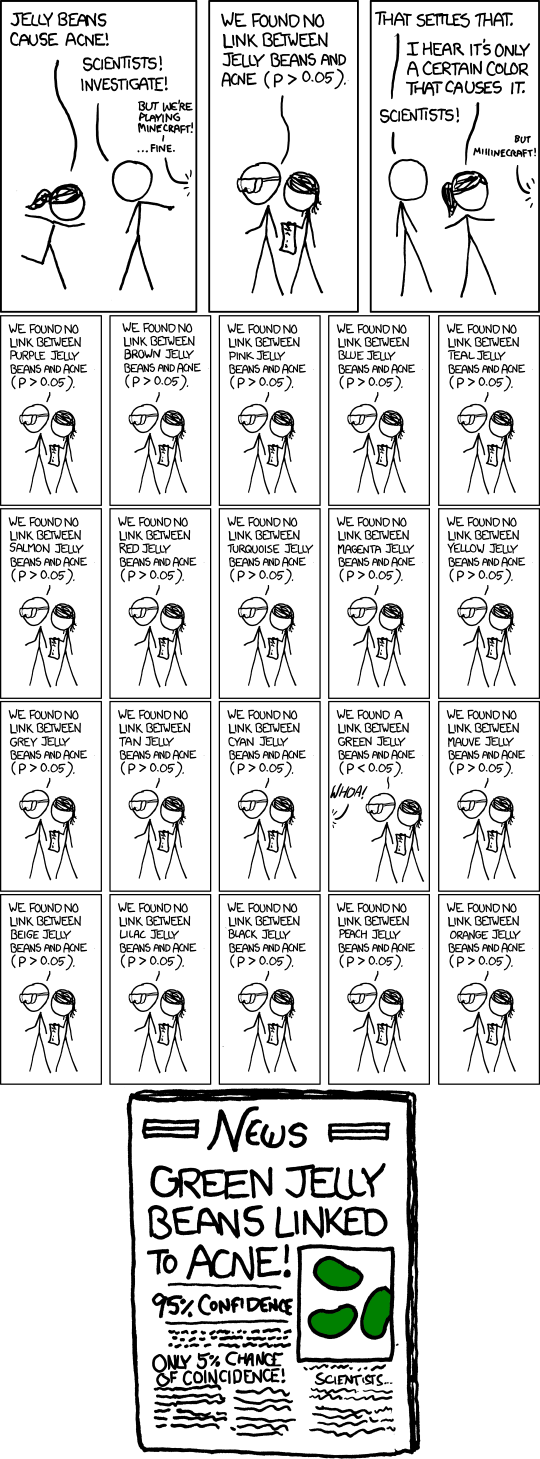
\includegraphics[width=0.46\textwidth]{figures/searches_significant_shrink.png}
\\
\begin{footnotesize}
`So, uh, we did the green study again and got no link. It was probably a{-}{-}'
\\
`RESEARCH CONFLICTED ON GREEN JELLY BEAN ACNE LINK; MORE~STUDY~RECOMMENDED!'
\end{footnotesize}
\caption[
``Significant'' from xkcd by Randall~Munroe
]{%
``Significant'' from xkcd by Randall~Munroe~\cite{xkcd2011significant}.
}
\label{fig:searches_significant}
\end{figure}

Neyman and Pearson formalized this \pvalue\ based suspicion into decision
rules and thought about what it is that makes one test statistic better than
another~\cite{neymanpearson1928max, neymanpearson1933lemma}.
Rather than a \pvalue\ arousing suspicion of an hypothesis, here it is used
to decide on actions of `rejecting' or `accepting' an hypothesis.
From the Bayesian arguments that we are presenting in
Section~\ref{sec:searches_data_analysis},
Neyman and Pearson argued for the interest in likelihood ratios, and further
considered their use as test statistics~\cite{neymanpearson1928max};
they also considered \emph{maximum} likelihood ratios
\begin{equation}
\label{eqn:searches_max_like_ratio}
\Lambda =
\frac{L(h_1)}{\mathrm{max}_i\,L(h_i)}
\end{equation}
for a specified hypothesis $h_1$ against the largest likelihood from a set
of alternatives.

As descriptions of the likelihoods in play, maximum likelihood ratios can
usefully communicate relevant information from the data.
And ass test statistics, they also win generality by avoid context-specific
motivations, such as scale invariance for the $t$-statistic of
Equation~\ref{eqn:searches_t_statistic} --- any situation with predictive
models can construct likelihoods and maximum likelihood ratios.
``Without claiming that this method is necessarily the ``best'' to adopt,''
Neyman and Pearson suggest maximum likelihood ratios as
``one clearly defined method of discriminating between samples for which
Hypothesis A is more probable and those for which it is less probable''~\cite{
neymanpearson1933lemma}.
To this quote, Lehmann appends ``(sic!)''~\cite{lehmann2011fisher}, since it
appears to conflate the likelihood for an hypothesis with its probability.
But Neyman and Pearson's association of likelihood ratios with
``more probable'' hypotheses may not be an error.
The authors understood the algebra of how large likelihood ratios make
hypotheses \emph{more probable} by changing their posterior probabilities,
independent of whatever (non-zero) prior probabilities they are assigned.
Indeed, they later state that
\begin{displayquote}
``%
The statistician can balance the numerical verdict of likelihood against the
vaguer expectations derived from `a priori' considerations, and it must be left
to his judgment to at what point the evidence in favour of alternative
hypotheses becomes so convincing that Hypothesis A must be rejected.%
''~\cite{neymanpearson1933lemma}
\end{displayquote}
Elsewhere also, they consider an example with two hypotheses $\mathrm{A}_1$
and $\mathrm{A}_2$, and find a $\log$ likelihood ratio of
% the two corresponding densities at the sample point are
% ($\mathrm{A}_1$) $6.42 \times 10^{-20}$,
% ($\mathrm{A}_2$) $5.18 \times 10^{-4}$ and the ratio of the likelihood of
% Hypothesis $\mathrm{A}_1$ to that of $\mathrm{A}_2$ is $1.24 \times 10^{-16}$.
$-37$, concluding that
``%
This ratio confirms the common-sense judgment that $\mathrm{A}_2$ is far more
plausible than $\mathrm{A}_1$%
''~\cite{neymanpearson1928max},
which again relates the likelihood ratio to how plausible an hypothesis is.

\begin{figure}[tp]
\centering
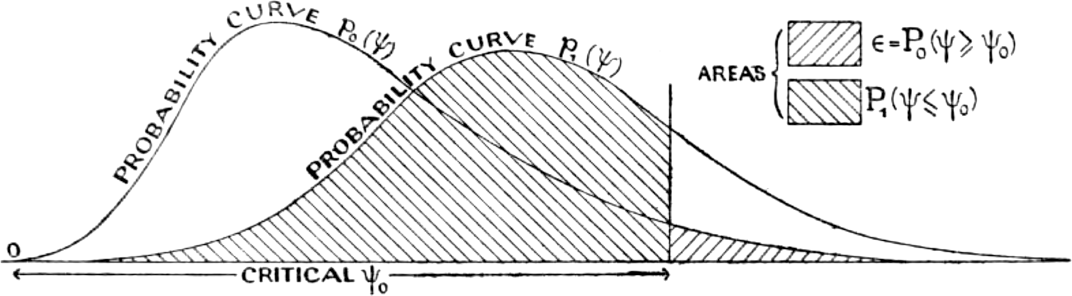
\includegraphics[width=0.95\textwidth]{figures/searches_np_curves_crop.png}
\caption[
Tail areas of prior probability distributions for data from two alternative
hypotheses, reproduced from Neyman and Pearson
]{%
Tail areas of prior probability distributions for data from two alternative
hypotheses, reproduced from Neyman and Pearson~\cite{neymanpearson1933lemma}.
}
\label{fig:searches_np_tails}
\end{figure}

The famous Neyman-Pearson lemma does not prove the usefulness of likelihood
ratios in probability algebra.
That was already known.
What it contributes is a relationship with one-sided inequalities ---
it states that likelihood ratios (not maximum likelihood ratios)
are optimal in a specific sense within their framework of decisions
based on $p$-values.
Precisely, at a fixed probability $\alpha$ of rejecting a true hypothesis,
the Neyman-Pearson lemma finds that a likelihood ratio test statistic maximizes
the probability $\alpha'$ of rejecting the alternative, false hypothesis that
lives in the denominator of the ratio; they illustrate this construction with
the diagram reproduced in Figure~\ref{fig:searches_np_tails}.

Only the likelihood ratio local to the observed data matters directly in the
probabilistic analysis, but this lemma is useful in the construction
of event variables of the kind we use in \atlas\ searches.
This can be seen from the signal and background distributions of
Figures~\ref{fig:searches_sig_bkg_prior_likelihood}
and~\ref{fig:searches_atlas_higgs_4l};
the event variable in Figure~\ref{fig:searches_sig_bkg_prior_likelihood} is
like a likelihood ratio in that any right-handed inequality selects a good
signal purity relative to its background yield, but the signal bump in the
middle of the background distribution in
Figure~\ref{fig:searches_atlas_higgs_4l} would be better selected with a
window around the Higgs boson mass.
Re-ordering $m_{4\ell}$ by a likelihood ratio could turn this selection window
into an equivalent and simpler one-sided selection, and the Neyman-Pearson
lemma states that there is no ordering that further optimizes the selected
signal-to-background ratio.

Neyman and Pearson were also involved in the development of
`confidence intervals', which are ranges of parameters that are
accepted by the \pvalue\ decision rules~\cite{
clopper1934confidence,
neyman1935Intervals,
Neyman1937Outline
}.%
\footnote{%
Confidence intervals are usually introduced by endpoints containing constrained
probability mass, but this \pvalue\ form can always satisfy that through the
free choice of test statistic and extends naturally beyond one dimension.%
}
A parameter corresponds to an hypothesis that assigns a prior distribution to
plausible data, and those data for which an obeisant researcher accepts the
hypothesis have probabilities that sum to $\gamma = 1 - \alpha$.
This $\gamma$ is known as the `confidence level'.
Such a rule selects a set of favoured data for each hypothesis, and the
confidence interval (when it can be constructed) contains hypotheses for which
the observed data are in that favoured set.

Confidence intervals are confusing.
It is easy to be tricked into thinking that the confidence interval for given
data `probably' contains the unknown parameter, but that gets it backwards.
For a known true parameter $x$, the confidence intervals in random repeated
experiments will contain that $x$ with probability $\gamma$;
the interval makes a subtle statement about unknown alternative data for
known true parameters.
Confidence intervals can even exclude all plausible parameters~\cite{
pratt1961testing,
Jaynes1976intervals
}.
Pratt eloquently explains the correct interpretation of a confidence interval
by example:
\begin{displayquote}
\small
``%
A method yielding true statements with probability $.95$, when applied to your
experiment, yields the statement that your treatment effect is between $17$ and
$29$, but no conclusion is possible about how probable it is that your
treatment effect is between $17$ an $29$.%
''~\cite{pratt1961testing}.
\end{displayquote}
Neyman and Pearson never claimed otherwise; they did precise mathematics, and
confusion about their intervals arises externally~\cite{jaynes2003probability}.

Confidence intervals are functions of the data, so can inform vague inferences
if used as data for likelihood functions, just as we did to interpret Fisher's
\pvalue\ ratio as a likelihood ratio ---
an accurately constructed confidence interval $x_1\textrm{--}x_2$ has a
likelihood function
\begin{equation}
L(x) =
\left\{
\begin{matrix}
\gamma & \textrm{if}~x \in x_1\textrm{--}x_2, \\
1 - \gamma & \textrm{otherwise.} \\
\end{matrix}
\right.
\end{equation}
And again, this reduction cannot add to the data.
It can only detract.
The recommendation by Fisher to directly communicate the likelihood function
remains simpler and clearer.
In response to the idea that no conclusion can be drawn about the parameter
itself, Fisher also deserves the last word:
\begin{displayquote}
\small
``%
There is something horrifying in the ideological movement represented by the
doctrine that reasoning, properly speaking, cannot be applied to empirical data
to lead to inferences valid in the real world.%
''~\cite{fisher1956statistical}
\end{displayquote}


\begin{singlespacing}
\section{Post-frequentist practice}
\label{sec:searches_practice}
\begin{epigraphs}
\qitem{%
\ldots\ But this book, by its very excellence, its thoroughness, lucidity and
precision, intensifies my growing feeling that nevertheless the theory is
arbitrary, be it however ``objective,'' and the problems it solves, however
precisely it may solve them, are not even simplified theoretical counterparts
of the real problems to which it is applied.%
}%
{John~W.~Pratt,
\textit{Review: Testing Statistical Hypotheses},
1961~\cite{pratt1961testing}}
\end{epigraphs}
\end{singlespacing}

Data analysis in modern High Energy Physics does not exactly follow frequentist
ideology, but is a hands-on, practical, and evolving mixture that has adapted
to avoid some of the more glaring flaws.
We have seen in Section~\ref{sec:searches_data_analysis} how likelihood ratios
can clearly express our scientific interest in how well competing models
predict data, and how those likelihoods can be manipulated in probability
algebra.
We have also seen in Section~\ref{sec:searches_frequentist} how 20th century
writers championed likelihoods not on the data themselves but on inequalities,
forming \pvalues\ and confidence intervals in reductions that throw away
information and obfuscate the results.
This section reviews how these objects are applied generally in conventional
analysis at the LHC and specifically towards the \atlas\ search that this
thesis presents.

Misrepresentations of \pvalues\ (and other frequentist statistics) are
widespread and widely reported~\cite{
schervish1996p,
Cohen1994TheEI,
Amrhein2017TheEI,
goodman2008dirty,
greenland2016no,
Bernstein2016princess,
wagenmakers2007practical
}
in fields where they are not banned~\cite{Trafimow2015ban}.
For example, the false presentation as a ``probability of compatibility'' with
a model~\cite{HIGG-2018-04} appears to be spreading as a good
meme~\cite{dawkins1989selfish} in High Energy Physics ~\cite{
HIGG-2017-09,
HIGG-2018-27,
HIGG-2018-51,
EXOT-2018-08,
HION-2018-19,
mastrandrea2019searches,
white2019search,
langford2021combination,
IceCube2013search,
IceCube2014searches,
gerasimov2021new
},%
\footnote{%
A draft of~\cite{HIGG-2018-51} stated that a \pvalue\ determined
``the probability that the background-only hypothesis is compatible with the
observed data''.
That text was removed in response to my internal comments, but
``probability of compatibility'' remains in its figure captions.%
}%
\footnote{%
Reference~\cite{HIGG-2018-57} accurately describes a \pvalue\ as a tail
probability, but also (repeatedly) states that a
``probability of compatibility\ldots\ corresponds to a \pvalue''.%
}%
and is plausibly explained by mutations from vaguely accurate statements like
``compatible with the SM prediction with a $P$ value of $0.10\%$''~\cite{
lhcb2021test
}
to precisely inaccurate statements like
``a probability of around $0.1\%$ that the data is compatible with the
Standard Model predictions''~\cite{cern2021test}.

There also exists a notion that a small \pvalue\ means that the data
represent a rare fluctuation~\cite{murray1997use, atlas2022pvalue}.%
\footnote{%
The \atlas\ Glossary of Terms~\cite{atlas2022pvalue} falsely states that
``The \textbf{p-value} is the probability (ranging from $0$ to $1$) that the
results observed could have occurred by chance, if the tested theory has no
impact on the study.''%
}
All \pvalues\ are rare.
By construction, they are uniformly distributed between $0$ and $1$, so the
probability that $P(h) < \varepsilon$ is equal to the probability that
$0.4 \leq P(h) < 0.4 + \varepsilon$ or that it lands in any
$\varepsilon$-sized set
(if the data are indeed sampled under $h$).
What matters to our interpretation is whether an alternative hypothesis
makes the observed result \emph{more probable}.

\subsection{\texorpdfstring{$\cls$}{CLs}}
Such misrepresentations of our results reinforces the need for clearer
replacements, which $\log$ likelihood ratios can provide.
And standard practice at the LHC contains the beginnings of such
replacements under the name $\cls$~\cite{
read2000modified,
Read2002cls,
junk1999confidence,
read1997optimal,
bock1998lower,
etde1998prospects,
lep2000searches,
lep2003search,
Murray2010heretic,
cern2011procedure,
pdg2022ynf
},
which is used for setting upper limits on disfavoured signal yields $s$
above background yields $b$;
\begin{equation}
\label{eqn:searches_cls}
\cls
=
\frac{P(s + b)}{P(b)}
=
\frac{
\prob{t \geq \tilde{t}}{s + b}
}{
\prob{t \geq \tilde{t}}{b}\hphantom{s +\;}
}
,
\end{equation}
in which the individual \pvalues\ are named
$\clb = P(b)$ and
$\clsb = P(s + b)$.%
\footnote{%
Despite the $\mathrm{CL}$ labels, these ($\cls$, $\clsb$, and $\clb$) are
not confidence levels ---
a confidence level $\gamma$ is a decision boundary used, for example,
to assign limits by solving for $x$ such that
$\gamma = 1 - P(x)$~\cite{pdg1996}.
In particle physics, \pvalues\ have sometimes been labelled $\mathrm{CL}$ since
at least 1984~\cite{pdg1984}, although textbooks from the '70s (which are cited
by~\cite{pdg1984}) do make the distinction~\cite{
eadie1971statistical,
frodesen1979probability
}.%
}%
\footnote{%
Some literature defines $\clb = 1 - p_b$~\cite{
Cowan:2010js,
pdg2022ynf
}, but such a $p_b$ might not be a \pvalue\ when it excludes equality with the
observed test statistic~\cite{cern2011procedure}.
}%
As discussed in Section~\ref{sec:searches_fisher}, \pvalues\ are likelihoods
on obfuscated data, so (with some caution) $\cls$ can be interpreted as a
likelihood ratio.%
\footnote{%
Likelihood ratios are useful if both their numerator and denominator use the
same data, so $\clsb$ and $\clb$ should use the same test statistic.
Identical test statistics are used for all results of this work, but differing
test statistics have been allowed elsewhere~\cite{bock1998lower}.
}%
At a given confidence level $\gamma$ (typically $95\%$), limits are set to
values of $s$ for which $\cls = 1 - \gamma$.

\begin{figure}[tp]
\centering
\begin{subfigure}{\textwidth}
\centering
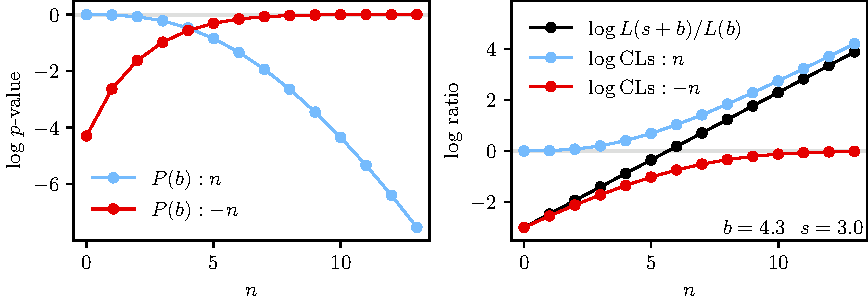
\includegraphics[width=\textwidth]{figures/searches_cls_plots_with_pvals_n.pdf}
\end{subfigure}
\caption[
A Poisson model in the natural order
]{%
A Poisson model in the natural order of $t(n) = \pm n$
test statistics, $b = 4.3$ and $s = 3.0$.
(left) $\log$ \pvalues,
and (right) $\log$ likelihood ratios and $\log$ $\cls$ for
background and signal-plus-background models.
The $n$ test statistic is Neyman-Pearson optimal because it is monotonically
(linearly) related to the likelihood ratio.
Each $\cls$ is a \pvalue\ ratio.
By reducing the observed data to an inequality, the $p$-value selectively
censors some of its information.
}
\label{fig:searches_sb_n}
\end{figure}

Early variants of $\cls$ derived it from an identity with posterior tail
probabilities in Poisson or Gaussian special cases~\cite{
Helene1983upper,
pdg1988,
read2000modified,
pdg2022ynf
}
with a contrived frequentist interpretation~\cite{zech1988cls}.
For use in general cases, it is more recently described as a
``modified frequentist'',
``approximate confidence in the signal-only hypothesis''~\cite{
read2000modified,
Read2002cls
}.
High-profile usage in Higgs boson searches at the
Large Electron–Positron Collider~\cite{
read1997optimal,
bock1998lower,
etde1998prospects,
junk1999confidence,
lep2000searches,
lep2003search
}
appears to have propelled $\cls$ to prominence;
these early applications used data deficits to exclude their
background-plus signal models, sometimes with the test statistic $t(n) = -n$,
and disliked how deficits led to small \pvalues\ for the background-only model,
with which they might have confusingly set negative limits on the Higgs boson
signal cross-section.
Such \pvalues\ are illustrated in Figure~\ref{fig:searches_sb_n} (left)
for small data counts;
in contrast, $\cls$ can only favour the background-only model, due to its
negative values that are shown on the right of the same figure.

Despite the statement in Section~\ref{sec:searches_fisher} that \pvalue\
ratios are not ``not \emph{necessarily} misleading'',
Figure~\ref{fig:searches_sb_n} shows a bias from the fact that
no data can give a $\cls$ that favours the signal model;
$\log\cls$ is non-positive with the $-n$ test statistic, and indeed non-negative
for the opposite ordering $t(n) = n$.
The $\log$ likelihood ratio on the actual data does not feature this bias:
it favours background-only for deficits and background-plus-signal for
excesses.
Since for Poisson models the $\log$ likelihood ratio is linear in $n$,
\begin{equation}
\log \frac{L(s + b)}{L(b)}
= n\log\frac{s + b}{b} - s
,
\end{equation}
both $n$ and $-n$ can be optimal in the Neyman-Pearson sense.

By using \pvalue\ ratios with Neyman-Pearson optimal test statistic, we have
constructed an analysis that can only ever favour one hypothesis:
we have built a propaganda machine that only ever speaks truth but censors any
information that supports alternative ideas.
Reducing data to inequalities $t \geq \tilde{t}$ implements the censorship,
and the likelihood-ratio ordering guarantees the one-sided inferences
that appear in Figure~\ref{fig:searches_sb_n} (right) as one-sided
$\log\cls$ values.

\begin{figure}[tp]
\centering
\begin{subfigure}{\textwidth}
\centering
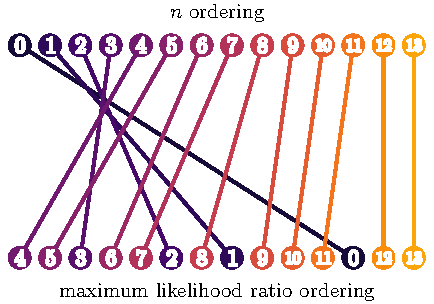
\includegraphics[width=0.5\textwidth]{figures/searches_cls_plots_with_pvals_order.pdf}
\caption{%
Ordering the data by a maximum likelihood ratio test statistic with $b=4.3$.
}
\end{subfigure}
\\[.5em]
\begin{subfigure}{\textwidth}
\centering
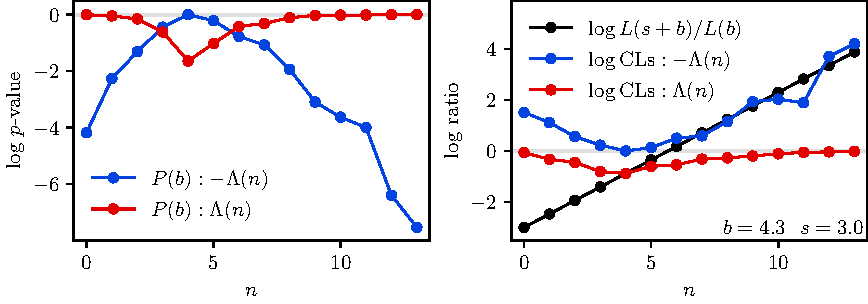
\includegraphics[width=\textwidth]{figures/searches_cls_plots_with_pvals_t.pdf}
\caption{%
(left) $\log$ \pvalues\ for Poisson data,
and (right) $\log$ likelihood ratios and $\log$ $\cls$ for
background and signal-plus-background models.%
}
\end{subfigure}
\caption[
Analysis of a minimal Poisson model with maximum likelihood ratio
test statistics
]{%
Analysis of a minimal Poisson model with maximum likelihood ratio
test statistics $t(n) = \pm \Lambda(n)$,
where $\Lambda(n) = L(b)/\mathrm{max}_x\,L(x)$; $b = 4.3$ and $s = 3.0$.
This test statistic jumbles up the data into an that makes $n=11$ appear to be
weaker support for the signal than $n=9$.
Each $\cls$ is \pvalue\ ratio.
By reducing the observed data to an inequality, the $p$-value selectively
censors some of its information.
}
\label{fig:searches_sb_t}
\end{figure}

How can one escape this propaganda?
Likelihood ratios on the actual data escape immediately by bypassing the
censor.
Even inequalities need not be biased --- if taken against a predetermined
threshold, say $5$ events, then models can predict whether $n \leq 5$,
and its truth or falsehood in data can favour either side.%
\footnote{%
This context of a fixed inequality is one condition where the
\pvalue\ ratio is not misleading when interpreted as a likelihood ratio.%
}
Finally, a reader can fall back to not trusting the reporter ---
the statements `\atlas\ reports $n \leq 5$' and logical `$n \leq 5$' are not
identical, since one can infer from the former that in fact $n = 5$.
One knows what the message says, but not that it states the whole truth.

With more than one Poisson bin to model, the $n$ test statistic is no longer
sufficient.
In such general cases, maximum likelihood ratio test statistics,
such as $\Lambda$ of Equation~\ref{eqn:searches_max_like_ratio}, often useful.
In the single Poisson case, $\Lambda$ shuffles the ordering of
data and leads to some odd features in the results, which are displayed in
Figure~\ref{fig:searches_sb_t}.
In particular, the choice $t(n) = -\Lambda(n)$ pushes data that are far from
the background expectation into its tails, so can disfavour the background
model for small $n$.
Probability masses from small data also interrupt its behaviour for excesses,
leading to jagged changes, notably that $\log\cls$ reduces as the data
increase from $9$ to $11$ --- counter to intuition and logic, increasing excess
data can reduce the reported favour for the signal model.

Instead of $\Lambda$ itself, various modified maximum likelihood ratio test
statistics enjoy standard usage at the LHC~\cite{cern2011procedure};
these are variably defined as piecewise functions of the fitted signal
parameter $s$, and can include likelihoods from the signal-plus-background
model with constrained maximizations which aim to reduce the impact of
unphysical results such as negative Poisson expectations~\cite{
Feldman:1997qc,
Cowan:2010js
},
and can improve (in a context-dependent sense) the resulting ordering.

These modified maximum likelihood ratios benefit from known approximations to
their sampling distributions in asymptotic (Gaussian) limits,
which can assign their \pvalues\ through well-behaved analytic
expressions~\cite{Cowan:2010js}.
Without such formulae, the remaining practical approach to estimating
\pvalues\ is to generate Monte Carlo simulations of alternative data.
Such simulations can be computationally expensive, ill-defined for
``likelihood'' models that blur the distinction between actual data and
auxiliary constraints on the models' parameters.


\subsection{Like-lihood modelling}
To represent the Standard Model and alternatives, LHC data analysis uses
parametric models to describe the models' Poisson expectations of
collision events and how those expectations change in response to their
parameters.
Parameters often correspond to interpretable, physical quantities and when
those parameters are known only with some uncertainty, the models help to
propagate uncertainty into variations of their outputs.

Uncertainties on imperfectly-known yet non-random parameters, however,
conflict with the frequentist denial of prior probabilities.
To avoid this, all modelling is officially framed as not predicting parameters,
but instead constraining them with likelihood functions that use
either real control data or fictional auxiliary data.

This transformation of priors to auxiliary likelihoods is generally possible
--- in a prior density $f(x)\,\mathrm{d}x$ the function $f(x)$ is a likelihood
(strictly, a Radon-Nikodym derivative~\cite{billingsley2008probability})
that constrains the (possibly non-normalized or `improper') prior measure that
is uniform in $x$~\cite{Cowan:2010js}.
But as discussed in Section~\ref{sec:searches_probability_applied}, the shape
of $f(x)$ is entirely determined by the coordinate, and is therefore a free
choice made by the analyst.
By assigning a form to the auxiliary likelihood, therefore, one is really
choosing a \emph{regularizer} that should be intended to induce preferable
behaviours in the parametric model and its `maximum likelihood' statistics.

These regularized models with constraints from fictitious auxiliary data
are usually often ``likelihood'' models~\cite{
cranmer2012histfactory,
baak2015histfitter,
Besjes_2015,
heinrich2021pyhf
}.
To distinguish them from real likelihood functions on actual data, this
thesis uses the alternative spelling \textbf{\heplikelihood}.

Many of our uncertainties do not correspond to predictions of auxiliary data:
examples include
scale variations,
theoretical cross-section uncertainties,
non-closure uncertainties (which cover differences between estimates),
simulated sample comparisons,
statistical errors on weighted simulations,
extrapolation uncertainties,
and
all uncertainties on supersymmetric signal yields
(for which we have yet no data).
We describe these uncertainties by heuristically
combining theoretical modelling, physical intuition, and convention,
and not only by measuring random data.
Believing that they are also likelihoods on auxiliary data is
doublethink~\cite{orwell1949nnineteen}.

Despite their troublesome nomenclature, \heplikelihood\ models are extremely
useful and effective for describing the predictions of our hypotheses and
extracting interpretable results.
A general \heplikelihood\ model is a function $H$ that takes some parameters $x$
and outputs two things:
expected yields $y$ to predict Poisson data,
and an objective value $E$ that should be minimized in a `fit' to choose the
best prediction.
That is,
\begin{equation}
H(x) = [\,y(x), \,E(x)\,]
.
\end{equation}
The minimization objective $E$ is the summed negative $\log$ likelihood
(or regularizer) for all actual and auxiliary data;
we choose the letter $E$ for \textbf{energy}, to highlight the analogy with
statistical physics and the Boltzmann factor
\begin{equation}
p(x) \propto e^{-\beta E(x)}
.
\end{equation}
with which a system collapses to its minimum energy at low temperature
$T = 1/\beta$.
At unit temperature, the Boltzmann factor can define a probability distribution
for the parameters relative to an appropriate (prior)
measure~\cite{cranmer2012histfactory, skilling2017david},
but in practice such distributions do not always coincide with intuition or
with the best fit value.

Error bars on the yields can be assigned by exploring around that best fit.
In the Gaussian approximation, the inverse (Hessian) matrix of second
derivatives gives a covariance matrix in the parameters from which linear
projections can estimate the variance of any output.
The second derivatives of exactly Gaussian forms are independent of the
parameter point, but since we do not have exactly Gaussian models we evaluate
these derivatives about the best fit point, either analytically or with finite
difference approximations~\cite{cranmer2021building}.
Other practical approaches explore parameter ranges in which the minimum energy
exceeds thresholds.

All results presented in this thesis use
\histfactory~\cite{cranmer2012histfactory} \heplikelihood\ models that are
constructed and analysed with
\histfitter~\cite{Besjes_2015,baak2015histfitter}
and \pyhf~\cite{heinrich2021pyhf}.
\histfactory\ models are specialized for working with discrete numbers of
histogram bins.
They constrain parameters with either Gaussian or Poisson%
\footnote{%
Poisson constraints typically use a continuous interpolation with
$n!\rightarrow \Gamma(n + 1)$.%
}
likelihood
functions, and assign expected yields through a variety of
non-linear functions of the parameters.
Each parameter's effect is generally described by
\emph{central}, \emph{high}, and \emph{low}
(corresponding to the best and $\pm1\sigma$)
values of modifications to bin yields.%
\footnote{%
Because extrapolations from the variations are non-linear, the exact forms of
the constraints do not directly matter.
Numerical optimizers prefer Gaussian forms for their $\log$ quadratic shape, which is
easily minimized in the common case that the parameter has no observable
effect.%
}

Along with each \heplikelihood\ constraint, \histfactory\ also assigns a
sampling distribution for alternative values of its (auxiliary) data.
To approximate \pvalues\ without the asymptotic approximations,
these distributions are used in a standard procedure for simulating
alternative ``pseudo-data (toys)''~\cite{cern2011procedure}.
This procedure works as follows:
\begin{enumerate}
\item fit to the observed data to find best-fit yields $\tilde{y}$, then
\item sample alternative Poisson (actual) data with rates $\tilde{y}$ and
alternative auxiliary (fictitious) data from their assigned distributions,
then
\item evaluate the test statistic for each simulated
example~\cite{cern2011procedure}.
\end{enumerate}
Because this first item fits to the observed data, the test statistic
distribution pathologically depends on the observed data $d$ ---
the approximated \pvalue\ is not
$\prob{t \geq t(d)}{h}$, but depends on the data like
$\prob{t \geq t(d)}{f(d, h)}$.
And since the \pvalue\ is a censored likelihood, this is an error of early
unblinding, or training on the test set in machine-learning speak.
It can make little difference when the yields are insensitive to the observed
data, but we shall see an example (of DR-Low) in
Section~\ref{sec:2ljets_results} where they are sensitive, and where
this makes a deficit in data appear much less significant than it should.
Sampling alternative data from exactly $\tilde{y}$, despite us actually being
uncertain of the expected yields
(demonstrated by us drawing error bars on them), is also suspicious.

Nonetheless, this procedure often simulates reasonable-looking test statistic
distributions without relying on the asymptotic approximations, and reportedly
has ``good coverage properties''~\cite{
cern2011procedure,
Cranmer2006Statistical
}.
Toy simulation is an alternative approximation, and in given circumstances
may be better or worse.
% Pick your poison.


\subsection{\atlas\ SUSY searches}
\label{sec:searches_searches}

\TODO{CR VR SR}


\subsection{Gaussian significance}

\TODO{significance}

% significance measures
The ATLAS-recommended significance measure~\cite{atlas_significance} is
\begin{align}
\label{eqn:significance_atlas}
S_\mathrm{\atlas}(n; \mu, \sigma) =~&
\sqrt{2} \times
\mathrm{sign}(n - \mu) \times
\\[0.2em] \nonumber
&
\sqrt{
n\log\left(\frac{n(\mu + \sigma^2)}{\mu^2 + n\sigma^2}\right)
- \frac{\mu^2}{\sigma^2}\log\left(
1 + \frac{\sigma^2(n - \mu)}{\mu(\mu + \sigma^2)}
\right)
}
,
\end{align}
taken in a limit where $0\log(0x) = 0$ for the $n=0$ case.
